\graphicspath{{./assets/}}
\setcounter{mtc}{11}
\chapter{9th Sprint: Disaster recovery }
\fancyhead[R]{\ungaramond\small\textbf{Chapter XI.   9th Sprint :Disaster recovery }}

\minitoc
\newpage
\section*{Introduction}
Disaster recovery is a critical aspect of any IT infrastructure, and Kubernetes environments are no exception. Kubernetes provides a resilient and scalable platform for deploying and managing containerized applications, but it is still vulnerable to various types of disasters such as hardware failures, data center outages, network outages, and human error. 

Disaster recovery in a Kubernetes environment involves planning and implementing strategies to ensure that the system can recover quickly and efficiently in the event of a disaster. This includes backing up critical data, deploying application components across multiple availability zones or regions, replicating data to off-site locations, and automating failover and recovery processes. 

In this chapter, we will cover disaster recovery planning, backup and recovery strategies, data replication, and automation.  


\section{Sprint backlog :}

\begin{longtable}[H]{|m{1.5cm}|m{3cm}|m{1.5cm}|m{9cm}|}
\hline
{\textbf{Epic ID}} & {\textbf{Epic}} & {\textbf{Story ID}} & {\textbf{Story}}\\
\hline
1  & Implement a resilient disaster recovery strategy.  &  1.1	 & Provisioning cloud storage resources. \\
\cline{3-4}
& & 1.2 & Preparing and applying a backup strategy for application specific data.  \\
\cline{3-4}
& & 1.3	& Preparing and applying a backup strategy for PaaS specific workloads.   \\
\cline{3-4}
\hline
\caption{9th Sprint Backlog}
\end{longtable}

\section{UML design: composite structure diagram of the disaster recovery strategy }

The following diagram describes the Disaster Recovery Strategy: 

\begin{figure}[H]\centering
    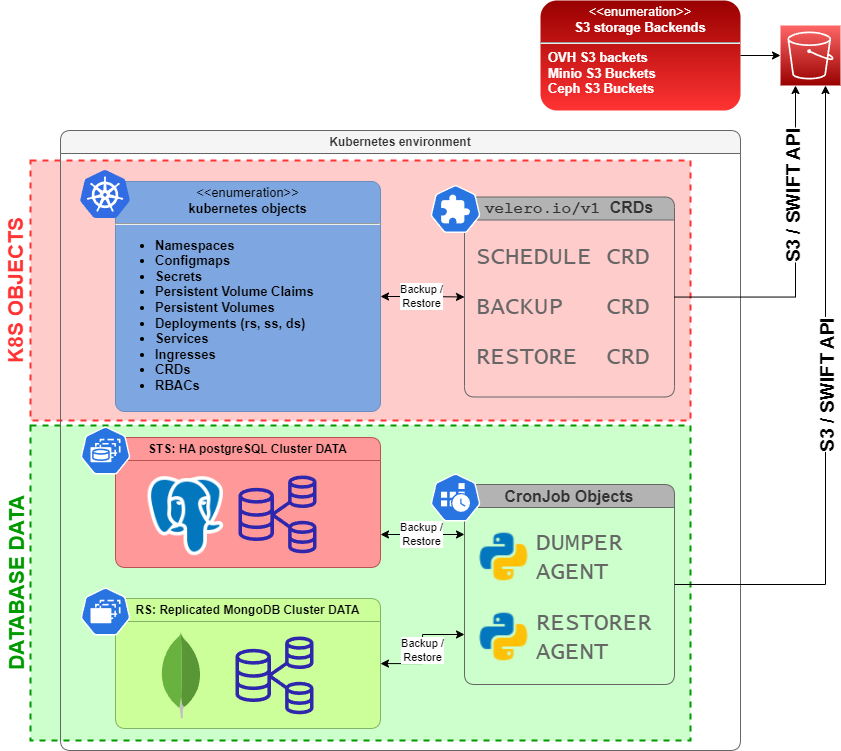
\includegraphics[width=1.0\textwidth,angle=00]{assets/f56.png}
    \caption{composite structure diagram of the disaster recovery strategy }
    \label{fig:f56}
\end{figure}

The disaster recovery relies on velero, a Kubernetes aware backup tool, and proprietary backup and restore containers written in python. 

Overall, this composite structure diagram shows how Velero and Kubernetes cronjobs work together to implement a disaster recovery strategy on Kubernetes that includes backing up and restoring both Kubernetes objects and database cluster data. 

\section{Disaster recovery for the PaaS environment }

As shown above in the composite structure diagram, velero is a powerful tool that enables us to backup and restore entire Kubernetes namespaces. 

 \subsection{Provider specific configurations }

Provisioning the object store containers that are destined to contain and serve backup data is dependent on the cloud provider. For the purpose of our strategy, we have written the following ansible role: 

\begin{listing}[H]
    \inputminted[firstline=1,lastline=34]{Yaml}{codeListing/role_openstack.yml}
\end{listing}

\begin{listing}[H]
    \inputminted[firstline=35]{Yaml}{codeListing/role_openstack.yml}
    \caption{Role Openstack}
    \label{lst:role openstack}
\end{listing}
This is an Ansible role that installs OpenStack and AWS CLI modules for Python, and sets up credentials for the AWS CLI. 

 

Deployment and configuration of the agent 

To facilitate backup and restore operations, this is the Ansible role responsible for installing the Velero client on Kubernetes master nodes and configuring it with AWS credentials: 

\begin{listing}[H]
\inputminted[firstline=1,lastline=41]{Yaml}{codeListing/role_velero.yml}
\end{listing}

\begin{listing}[H]
\inputminted[firstline=42]{Yaml}{codeListing/role_velero.yml}
\caption{Role velero}
\label{lst:role velero}
\end{listing}

Here's a breakdown of the role tasks: 
\begin{itemize}[label={--}]
\item The role starts by downloading and installing Velero client binary on the master nodes, then copying workspace contents to the server. Afterward, it installs Custom Resource Definitions (CRDs) for Velero and sets up Role-Based Access Control (RBAC) on the Kubernetes cluster. 
\item  The next step is to Base64 encode AWS credentials from the local “.aws/credentials” file, which will be used to create a Kubernetes secret for Velero. The encoded credentials are printed to the console for debugging purposes. 
\item Finally, the role creates a Velero secret from a Jinja2 template file using the encoded credentials and deploys the Velero client to the Kubernetes cluster. 
\end{itemize}
 

\subsection{Implementing backup and restore operations }

The backup and restore operations of the various Kubernetes objects are initiated by the operator either manually or using an ansible playbook tailored specifically for our PaaS. 

 \begin{figure}[H]\centering
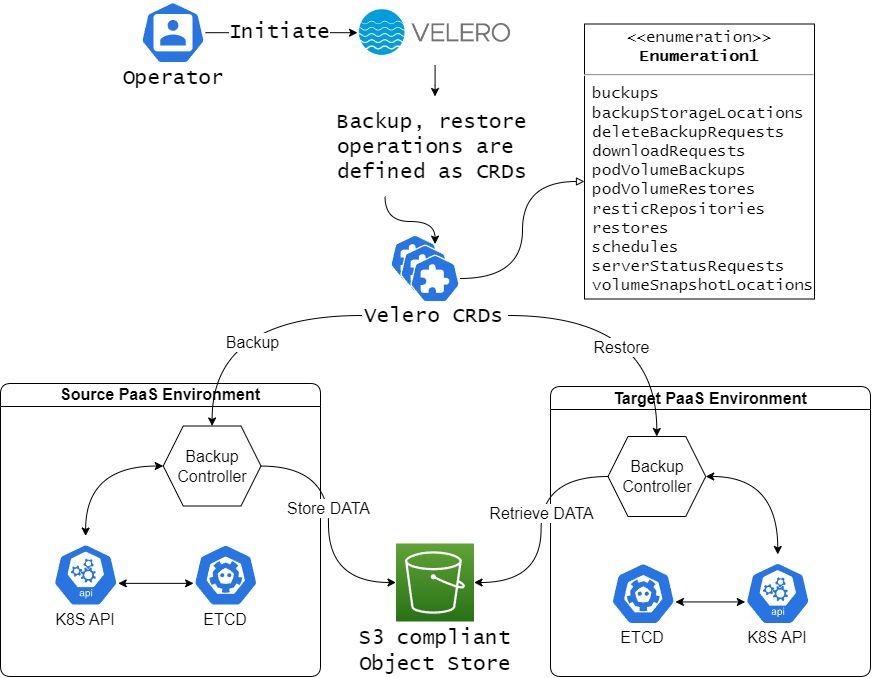
\includegraphics[width=1.0\textwidth,angle=00]{assets/f57.png}
\caption{Architecture of kubernetes objects Backup }
\label{fig:f57}
\end{figure}

As illustrated in the architecture above, the deployed Velero controller communicates with the Kubernetes API server to identify resources that need to be backed up or restored. In case of a backup operation, it stores backup data in an object store. This data is then retrieved to be restored. 

 

\section{Disaster recovery for the Database servers }

Only backing up persisted Kubernetes objects is unfortunately insufficient. In Kubernetes, backing up volumes that contain a database's data is not recommended because it can lead to inconsistent data being backed up. When a backup of a volume is created while the database is still running and actively writing to the volume, the backup might include an inconsistent view of the data. This is because the backup process is not transactionally consistent with the database, meaning that the backup might capture changes that were in progress but not yet completed. 

To avoid this issue, it is recommended to dump the database data first. 

 \subsection{Programmatically backing up and restoring database data }

In order to eliminate the need for user intervention, we have developed a few python programs that are charged to efficiently perform backup and restore operations. 

\subsubsection{Backup agent for the replicated MongoDB cluster data: }

The following class diagram illustrates a Python script that creates a backup of a MongoDB database and uploads it to cloud storage or a local directory: 

 \begin{figure}[H]\centering
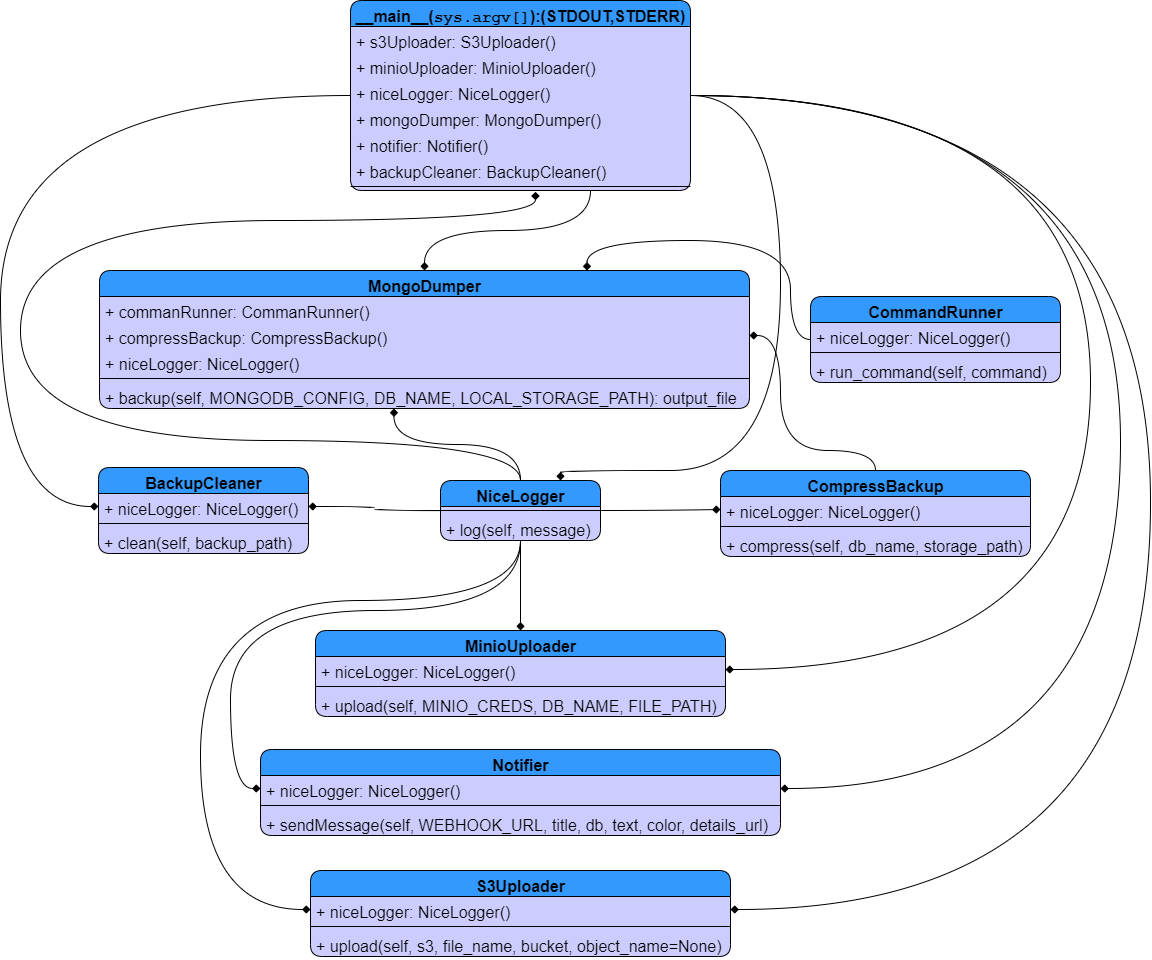
\includegraphics[width=1.0\textwidth,angle=00]{assets/f58.png}
\caption{Backup agent for the replicated MongoDB }
\label{fig:f58}
\end{figure}

The script collects MongoDB configuration parameters, such as the database host, port, username, and password, from the environment variables or configuration files. 

The script defines several classes, each of which has methods that perform specific functions: 

\begin{itemize}[label={--}]
\item “NiceLogger”: A logging utility that logs messages with timestamps. 
\item “BackupCleaner”: A class that contains a method to clean up old backups from the backup persistent volume. 
\item  “CompressBackup”: A class that contains a method to compress the backup  data. 
\item  “S3Uploader”: A class that contains a method to upload the compressed backup to AWS S3 cloud storage. 
\item “MinioUploader”: A class that contains a method to upload the compressed backup to MinIO cloud storage. 
\item  “Notifier”: A class that sends a notification message to Microsoft Teams. 
\item  “CommandRunner”: A class that runs shell commands. 
\item “MongoDumper”: A class that contains a method to create a MongoDB dump, compress it, and upload it to cloud storage. 
\end{itemize}
 

\subsubsection{Backup agent for the HA PostgreSQL cluster data: }

In a similar fashion to backing up the MongoDB cluster data, we have developed a backup agent for PostgreSQL. The following is the class diagram : 

\begin{figure}[H]\centering
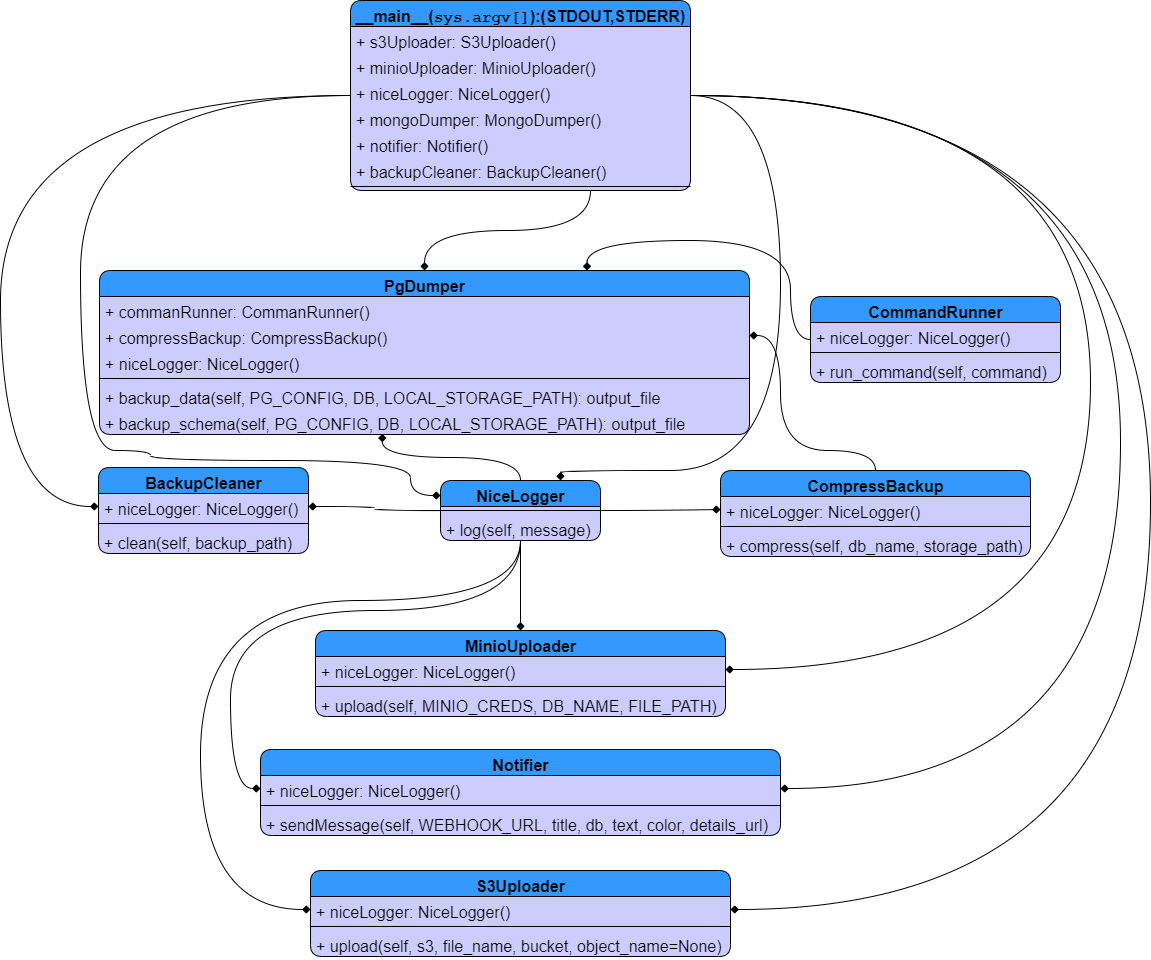
\includegraphics[width=1.0\textwidth,angle=00]{assets/f59.png}
\caption{Backup agent for PostgreSQL}
\label{fig:f59}
\end{figure}


PostgreSQL and MongoDB have different data storage architectures.  

When backing up PostgreSQL, it's important to back up both the data and the schema because the schema defines the structure of the tables and the relationships between them. Without the schema, it would be difficult to restore the database to its original state. 

\subsubsection{Restorer agent for the replicated MongoDB cluster data: }

This Python program is designed to restore a MongoDB database from the S3 Minio or AWS backups. 

\begin{figure}[H]\centering
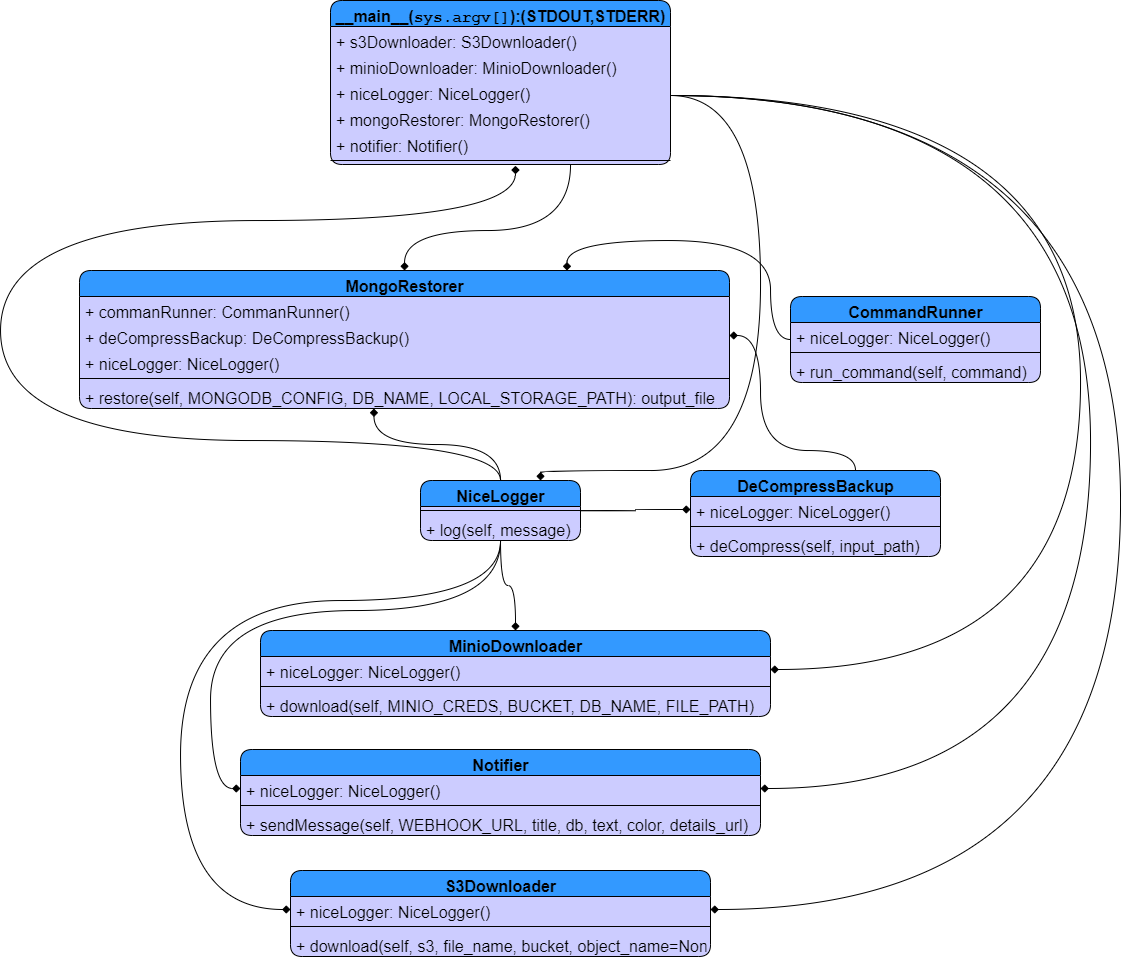
\includegraphics[width=1.0\textwidth,angle=00]{assets/f60.png}
\caption{Restorer agent for the replicated MongoDB }
\label{fig:f60}
\end{figure}

\subsubsection{Restorer agent for the HA PostgreSQL cluster data: }

The following is the class diagram for the python program responsible for restoring both data and PostgreSQL schemas: 

\begin{figure}[H]\centering
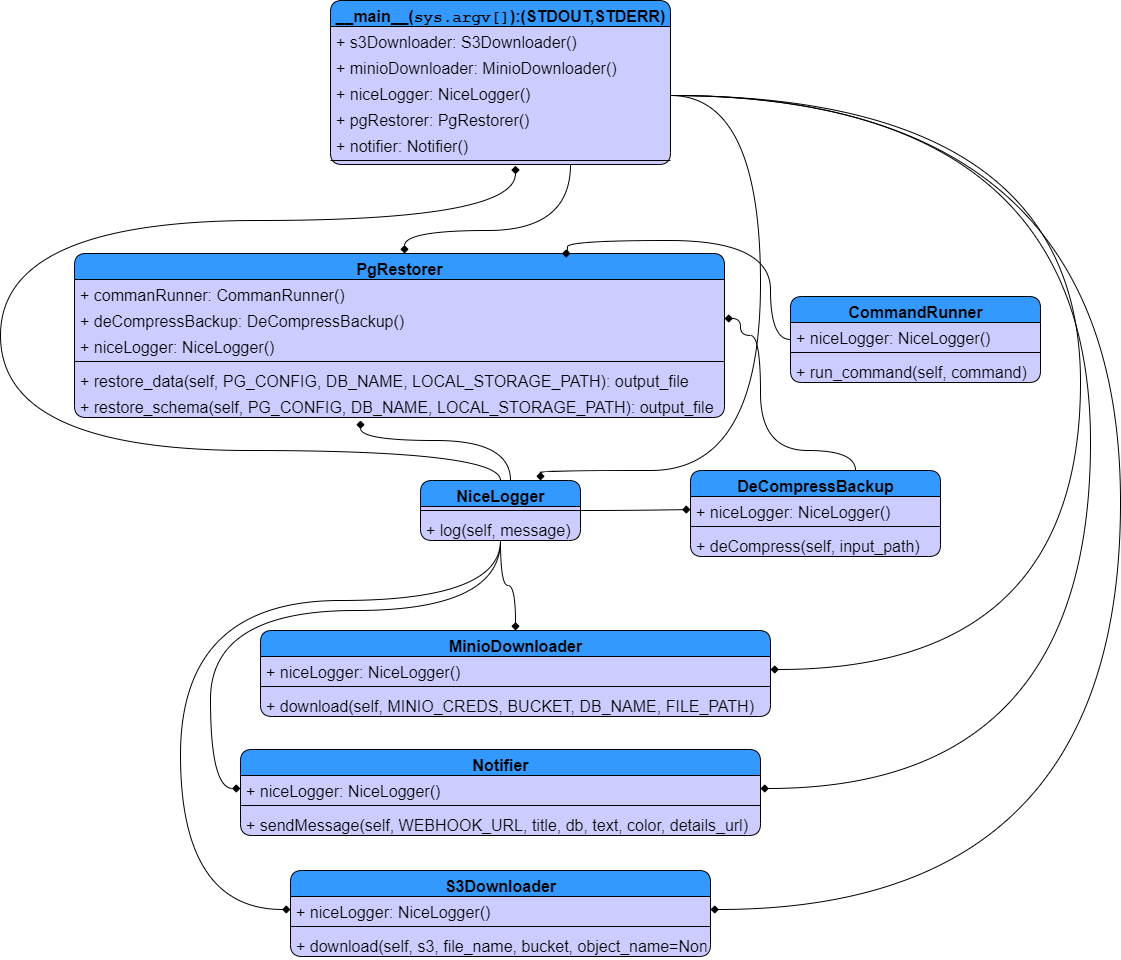
\includegraphics[width=1.0\textwidth,angle=00]{assets/f61.png}
\caption{Restorer agent for the HA PostgreSQL }
\label{fig:f61}
\end{figure}

\subsection{ Scheduling backup and restore jobs }

For each database cluster we have built a container image to which we then inject the python program responsible for backing up or restoring data. This is then used to configure a Kubernetes “CronJob” that runs periodically. The following is an example of the “CronJob” for backing up MongoDB: 

% \newpage
% \begin{multicols}{2}
% \begin{listing}
% \begin{multicols}{2}{}
    % \inputminted[firstline=1,lastline=40]{Yaml}{codeListing/cronjob_backup_mongo.yml}
    % \columnbreak 
    % \inputminted[firstline=41,lastline=80]{Yaml}{codeListing/cronjob_backup_mongo.yml}
    % \newpage
    % \inputminted[firstline=61,lastline=80]{Yaml}{codeListing/cronjob_backup_mongo.yml}
    % \columnbreak
    % \inputminted[firstline=81,lastline=100]{Yaml}{codeListing/cronjob_backup_mongo.yml}
% \end{multicols}
    % \caption{cronjob backup mongo}
    % \label{lst:cronjob backup mongo}
% \end{listing}
% \newpage
% \begin{listing}[H]
% \begin{multicols}{2}
% \inputminted[firstline=61,lastline=80]{Yaml}{codeListing/cronjob_backup_mongo.yml}
% \inputminted[firstline=81,lastline=100]{Yaml}{codeListing/cronjob_backup_mongo.yml}
% \end{multicols}
%     \caption{cronjob backup mongo}
%     \label{lst:cronjob backup mongo}
% \end{listing}
% \end{multicols}
% \newpage


\begin{listing}
\inputminted[firstline=1,lastline=50]{Yaml}{codeListing/cronjob_backup_mongo.yml}
\end{listing}

\begin{listing}
\inputminted[firstline=51,lastline=100]{Yaml}{codeListing/cronjob_backup_mongo.yml}
\end{listing}

\begin{listing}
\inputminted[firstline=71]{Yaml}{codeListing/cronjob_backup_mongo.yml}
 \caption{cronjob backup mongo}
    \label{lst:cronjob backup mongo}
\end{listing}

In this case, the CronJob is named "mongodump-demodb" and is defined in the "mongodb" namespace. 

These are some of the specifications: 
\begin{itemize}[label={--}]
\item “schedule: ‘0 0 4,12,20,28 * *’ ”: This defines the time and frequency at which the job will run, using a cron expression. In this case, the job will run at midnight, every 8 days of each month. 
\item  “concurrencyPolicy: Forbid”: This specifies how to handle overlapping job executions. With the "Forbid" option, if a job is already running at the time a new one is scheduled to start, the new job will not be run. 
\end{itemize}

Other than the environment variables to configure the backup program and the volume mounts to inject config files, we have attached a Persistent Volume from our distributed storage cluster to be able to backup data locally. 

Each of the python programs we have developed can back up and restore the entirety of the cluster data in one go. It only amounts to Setting the “DB\_NAME” environment variable to “NULL”. 

\section*{Conclusion}
Disaster recovery is a critical aspect of any PaaS environment that hosts mission-critical applications and services. The ability to recover from disasters quickly and efficiently can make the difference between a minor service disruption and a significant business failure. 

For Kubernetes-based PaaS environments, disaster recovery planning should include considerations such as data replication and backup, failover strategies, and hosting location redundancy.  

Similarly, for MongoDB and PostgreSQL database servers, disaster recovery planning should involve robust backup and restoration processes, as well as monitoring and testing procedures to identify and address potential points of failure.  

Ultimately, disaster recovery planning is an ongoing process that requires continuous monitoring and refinement. 